\begin{figure*}[!t]
    \centering
    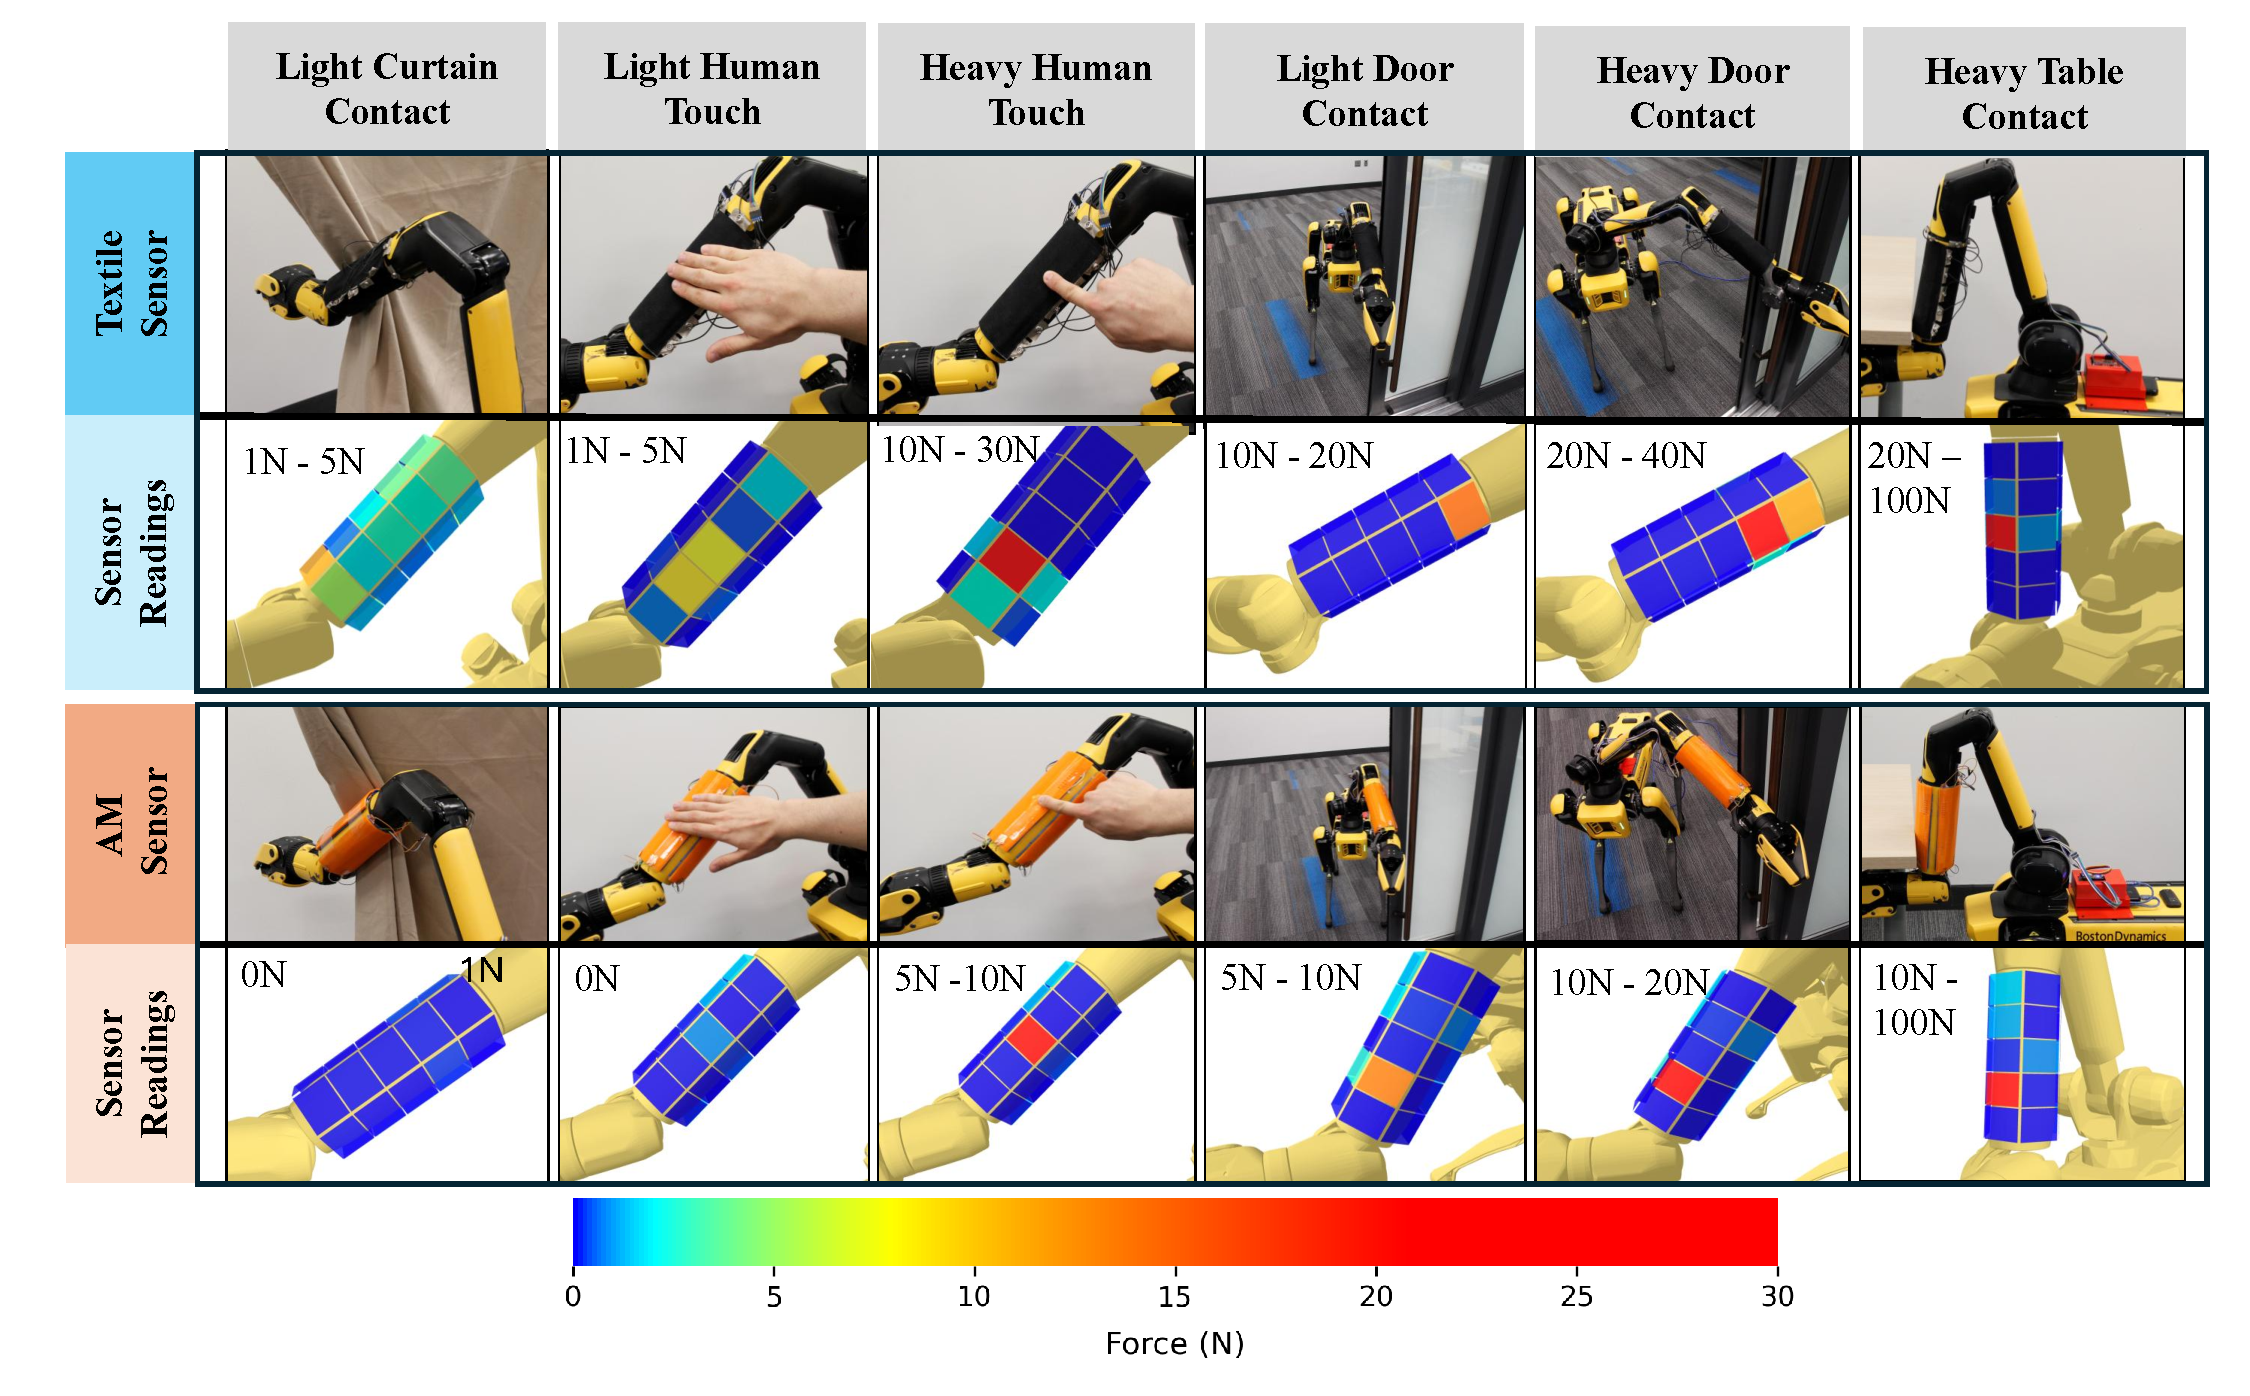
\includegraphics[width=1.0\linewidth]{images/Results_V7.pdf}
    \vspace{-0.5cm}
    \caption{Real-world deployment of the textile and AM sensors across representative manipulation scenarios. For each scenario, the middle panel visualizes tactile responses during contact, and the annotated values report the corresponding force ranges estimated from the sensor models. Upper bounds above 30~N are extrapolations beyond the 30~N calibration maximum and are included only to indicate the observed high-force regime.}\label{fig:results}
\end{figure*}

\section{Sensor Designs}




% \begin{table*}[t]
% \centering
% \scriptsize
% \setlength{\tabcolsep}{3pt}
% \renewcommand{\arraystretch}{1.10}
% \begin{tabular}{|p{3cm}|p{6cm}|p{6cm}|}
% \hline
% \textbf{Goal} & \textbf{Textile-based Sensor } & \textbf{Additive Manufacturing-based Sensor} \\
% \hline

% Shift force range downward (sense lower forces) &
% \tightitemize
% \item Thinner outer fabric
% \item Softer outer fabric
% \endtightitemize
% &
% \tightitemize
% \item Thinner outer material
% \item Softer outer material
% \item Decrease infill density
% \item Lower ridge height
% \endtightitemize
% \\
% \hline

% Shift force range upward (sense higher forces) &
% \tightitemize
% \item Thicker outer fabric
% \item Stiffer outer fabric
% \item Add spacer material (e.g., foam between outer fabric and electrodes)
% \endtightitemize
% &
% \tightitemize
% \item Thicker outer material
% \item Stiffer outer material
% \item Increase infill density
% \item Increase ridge height
% \endtightitemize
% \\
% \hline

% Expand force range &
% \tightitemize
% \item Add spacer material (e.g., foam between outer fabric and electrodes)
% \endtightitemize
% &
% \tightitemize
% \item Thicker outer material
% \item Add spacer material
% \endtightitemize
% \\
% \hline

% Narrow force range &
% \tightitemize
% \item No spacer material
% \endtightitemize
% &
% \tightitemize
% \item Thinner outer material
% \item Softer outer material
% \item Higher infill density
% \endtightitemize
% \\
% \hline

% Reduce hysteresis &
% \tightitemize
% \item Stiffer outer fabric
% \item Thinner spacer material or no spacer material
% \endtightitemize
% &
% \tightitemize
% \item Stiffer outer material
% \item Higher infill density
% \endtightitemize
% \\
% \hline

% \end{tabular}
% \caption{Design strategies for tuning force range and hysteresis in textile-based and 3D printed sensor arrays.}
% \label{tab:design_tuning_comparison}
% \end{table*}


Here we describe the sensor designs for the two architectures, tailored to the arm links of the Spot mobile manipulation platform. We design them to balance three practical requirements: (1) operating force range, (2) sensing repeatability across repeated load cycles, and (3) deployability on commercial robots through removable link-mounted skins rather than permanent link modification.

Both sensor designs share a common operating principle: a matrix of conductive rows and columns separated by a piezoresistive layer (Velostat). When contact occurs at a taxel, the piezoresistive layer compresses and becomes more conductive, changing the resistance at the row–column intersection, which is measured by a microcontroller through a voltage divider circuit. Both designs target link-level coverage, analog force readings across individual taxels, and fabrication with commercially available materials; the AM workflow uses robot-link meshes to adapt the shell geometry to a target platform.

We implement two complementary variants: (1) a textile-based sensor using conductive fabric layers, and (2) an additive manufacturing (AM) based sensor with 3D-printed conformal shells and copper-tape electrodes. We chose design variables such that the textile sensor prioritizes flexibility and lower-force contact response, while the AM sensor provides a conformal shell for higher-threshold contact. In these configurations, they support the two behaviors evaluated in Sec.~\ref{sec:results}: contact avoidance and contact embracing. We describe the design and fabrication of each in the following sections, with an overview shown in Fig.~\ref{fig:tactile_sensors_both}.
% \vspace{-5}
\subsection{Textile Sensor Design}
The textile sensor shown in Fig.~\ref{fig:tactile_sensors_both} is a flexible sleeve that mounts to the robot arm without rigid shells. Both the textile and AM sensors use a matrix of conductive rows and columns separated by a piezoresistive Velostat layer, with the same taxel pitch of approximately 20~mm. The sensor is formed into a cylindrical sleeve using hook-and-loop tape as a closure, allowing it to be wrapped around and removed from the robot link for maintenance. Rows and columns are interfaced with the microcontroller via snap buttons.

\begin{enumerate}[leftmargin=*]
\item \textbf{Inner layer:} The inner layer template is derived from a 2D projection of the robot link geometry and cut from a textured off-the-shelf fabric, chosen for flexibility and to reduce slipping against the robot surface. Rows of conductive fabric are adhered to the inner layer, with excess fabric removed at taxel boundaries to electrically isolate adjacent rows.
\item \textbf{Outer layer:} The outer layer uses the same template and also uses off-the-shelf fabric, providing a soft contact surface for improved sensitivity. Columns of conductive fabric are adhered to the outer layer, with excess fabric removed at taxel boundaries to isolate adjacent columns.
\item \textbf{Force Sensitive Layer:} Velostat squares are cut such that they are slightly wider than the conductive rows and columns to prevent short-circuiting.  
\item \textbf{Assembly:} The inner layer, Velostat squares, and outer layer are stacked in order and a fabric adhesive is used around each Velostat square to secure it. The sensor is then wrapped around the robot link, then secured with hook-and-loop tape. Snap buttons connect wires to each row and column, which are routed to a microcontroller.
\end{enumerate}
The fabrication of this sensor requires fabric cutting, ironing, adhesive, and snap-button wiring, and the material cost is less than $\$10$ per Spot arm link, excluding shared readout electronics.




\subsection{Additive Manufacturing (AM) Sensor Design}
The AM sensor is intended for tasks where direct textile wrapping is less appropriate: the skin must hold a repeatable shape on curved rigid links, avoid pre-compressing the sensing layer during installation, and respond primarily after a deliberate contact threshold is reached. A simpler taped or fabric-wrapped matrix can provide contact sensing, but its baseline response depends on wrap tension and local curvature. The printed shell instead fixes the electrode spacing and contact geometry relative to the robot link.

To design the 3D-printed skin, we start from the link-level mesh files provided by Boston Dynamics (Fig.~\ref{fig:tactile_sensors_both}-2, yellow) as part of their URDF models. The AM sensor uses the same 20~mm center-to-center taxel spacing as the textile sensor, but places the Velostat/copper-tape matrix inside a 95A TPU shell so that contact must first close a designed gap. The selected geometry was chosen to satisfy three constraints rather than to optimize over the full design space: maintain the same taxel spacing as the textile prototype, provide enough shell thickness and clearance for printable 95A TPU link covers, and create a mechanical threshold suitable for the contact-embracing task in Sec.~\ref{sec:results}. This geometry targets higher-threshold contacts than the textile sleeve while preserving link-level conformability. For each link, we apply the following sequence of CAD operations:

\begin{enumerate}[leftmargin=*]
\item \textbf{Inner layer:} Generate a conformal shell with a uniform thickness of 3~mm offset outward from the robot's base geometry (Fig.~\ref{fig:tactile_sensors_both}-2, green).
\item \textbf{Outer layer:} A second shell (\textit{3 mm} thick) offset \textit{5 mm} from the robot’s base geometry to accommodate the sensing stack (Fig.~\ref{fig:tactile_sensors_both}-2, orange).
\item \textbf{Ridges:} Within the inter-shell region, add 1~mm-thick horizontal ridges on the inner shell and vertical ridges on the outer shell, each 2~mm high. The spacing between adjacent ridges determines the taxel density (Fig.~\ref{fig:tactile_sensors_both}-2, cutout).
\item \textbf{Clearance cuts:} Material is removed near kinematic joints to prevent interference during motion, and a longitudinal cut is added along each shell to facilitate installation on the robot arm (Fig.~\ref{fig:tactile_sensors_both}-1).
\item \textbf{Assembly:} Print shells in 95A TPU. Laminate Velostat with copper tape (conductive adhesive), adhere to the inner shell, and apply copper tape to the outer shell for opposing electrodes. Connect rows/columns to the microcontroller and secure the assembled shells to the robot arm.
\end{enumerate}


 The fabrication of this sensor requires a 3D printer capable of printing flexible filaments, copper tape, Velostat, and wiring, and the material cost remains under \textit{\$10} per Spot arm link, excluding shared readout electronics. In the characterization protocol of Sec.~\ref{sec:characterization}, both sensors are tested over repeated 0--30 N load--unload cycles to measure operating force range, repeatability, and hysteresis.




\begin{figure}
    \centering
    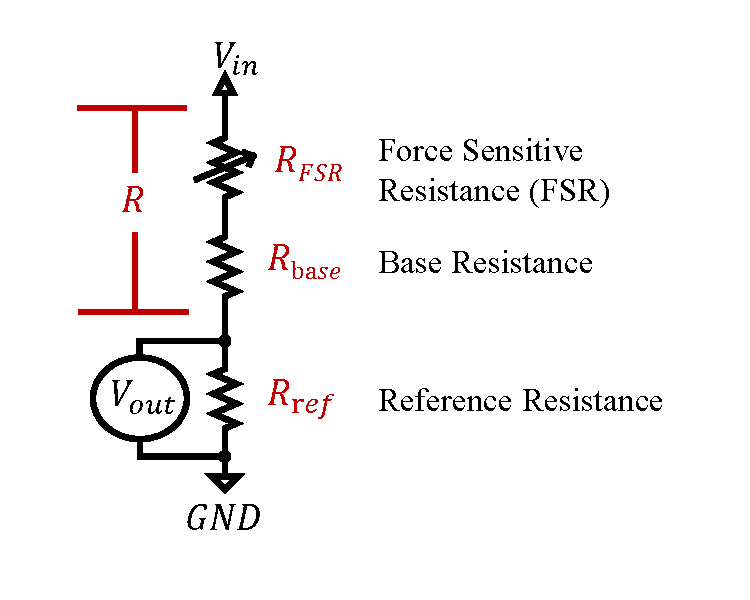
\includegraphics[width=0.75\columnwidth]{images/Circuit_v2.pdf}
    \caption{We model both of our sensors as a piezoresistive element in series with a base resistance. To measure the resistance of each element, we use a voltage divider and measure the voltage across a reference resistor. $V_{\mathrm{in}}$ and GND are GPIO from a microcontroller, where both are set to high-impedance after sampling to reduce cross-talk.}
    \label{fig:circuit}
\end{figure}




\subsection{Design Variables}

Both architectures expose practical design variables that can be adjusted to match task requirements for force range, repeatability, and fabrication effort. If only binary contact is required, the Velostat layer can be omitted; continuous force estimation requires retaining and calibrating the piezoresistive layer.

For the textile sensor, the principal variables are outer-layer stiffness and thickness, optional spacer material, and sleeve tension. Based on the sensor structure, softer or thinner outer layers are expected to shift the response toward lower contact forces, while thicker or stiffer fabrics should shift it upward; these effects were not independently swept in this study. A spacer material such as foam may broaden the response range, while minimizing the spacer may reduce hysteresis. Installation tension can also change pre-compression and the sensor's characteristic curve across deployments. The characterized configuration is configured for lower-threshold contact avoidance.

For the AM sensor, shell thickness, ridge height and spacing, material stiffness, and infill density determine the printed contact geometry. We characterize one configuration rather than a full parameter sweep. Lower shell stiffness, lower infill, or shorter ridges are expected to reduce the force needed to close the designed gap, while the opposite changes should increase the contact threshold. Ridge spacing sets taxel pitch, which is 20~mm in our prototype. TPU viscoelasticity and print structure may affect hysteresis, while the rigid-conformal shell reduces sensitivity to installation tension. Unlike the textile sensor's normally contacting stack, the AM sensor's designed gap closes only under compression, configuring it for higher-threshold contact-embracing tasks.
